\section{Esercizio 8 -- Comunicazione con handshaking}
\subsection{Esercizio 8.1}
L'obiettivo è progettare, implementare in VHDL e testare un sistema in cui due nodi (A e B) comunicano tramite un protocollo di handshaking [Figure \ref{fig:handshaking}, \ref{fig:8_1_HANDSHAKING}].

\begin{figure}[h]
    \centering
    \begin{minipage}[c]{0.45\linewidth}
        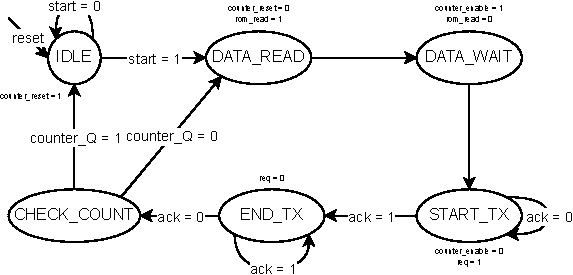
\includegraphics[width=\linewidth]{img/handshaking_A.pdf}
    \end{minipage}
    \hfill
    \begin{minipage}[c]{0.45\linewidth}
        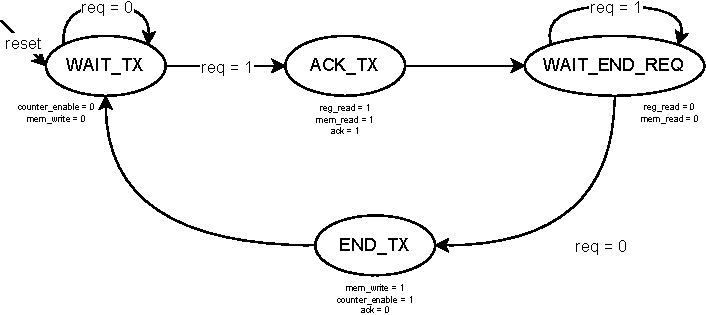
\includegraphics[width=\linewidth]{img/handshaking_B.pdf}
    \end{minipage}
    \caption{Automi dei sistemi A e B}
    \label{fig:handshaking}
\end{figure}

\begin{figure}[h]
    \centering
    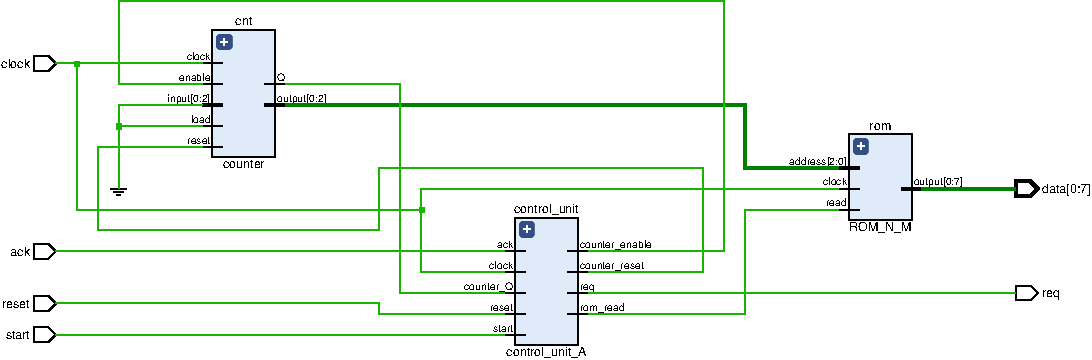
\includegraphics[width=\linewidth]{img/8_1_HANDSHAKING_A.pdf}
    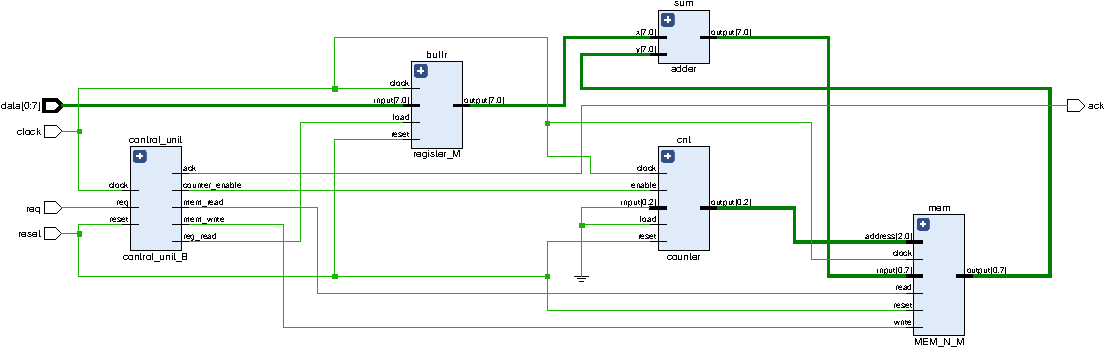
\includegraphics[width=\linewidth]{img/8_1_HANDSHAKING_B.pdf}
    \caption{Schema a blocchi del sistema di comunicazione con handshaking}
    \label{fig:8_1_HANDSHAKING}
\end{figure}

\subsubsection{Implementazione}
Si parte dal nodo A:

\begin{code}
    \inputminted{vhdl}{vhdl/handshaking_system_A.vhd}
    \caption{Implementazione del sistema A}
    \label{cod:handshaking_system_A}
\end{code}

\begin{code}
    \inputminted{vhdl}{vhdl/handshaking_control_unit_A.vhd}
    \caption{Implementazione dell'unità di controllo del sistema A}
    \label{cod:handshaking_control_unit_A}
\end{code}

\paragraph{Funzionamento generale.}
Il nodo A è responsabile della trasmissione delle stringhe $X(i)$ al nodo B utilizzando un protocollo di handshaking. Questo protocollo garantisce che ogni dato venga inviato e ricevuto correttamente prima di passare al successivo:

\begin{itemize}
    \item ROM Interna: il nodo A possiede una memoria ROM contenente $N$ stringhe di $M$ bit chiamate $X(i)$, che devono essere trasmesse al nodo B.
    \item Handshaking tra A e B:
    \begin{itemize}
        \item A invia un segnale di richiesta (\texttt{req = 1}) quando un nuovo dato è pronto.
        \item B risponde con un segnale di acknowledgment (\texttt{ack = 1}) quando ha ricevuto il dato.
        \item Solo dopo aver ricevuto \texttt{ack}, A procede con la trasmissione del prossimo dato.
        \item Questo processo continua finché tutte le $N$ stringhe sono state inviate.
    \end{itemize}
    \item Contatore per la trasmissione:
    \begin{itemize}
        \item A utilizza un contatore per gestire la sequenza di trasmissione.
        \item Il contatore scorre da 0 a $N-1$, leggendo ogni stringa $X(i)$ dalla ROM e inviandola a B.
        \item Quando il contatore raggiunge $N-1$, la trasmissione termina.
    \end{itemize}
    \item Unità di controllo: coordina l'intero processo gestendo i segnali di richiesta (\texttt{req}), acknowledgment (\texttt{ack}), lettura dalla ROM e incremento del contatore.
\end{itemize}

\paragraph{Struttura del codice.}
L’architettura è \texttt{structural} [Codice sorgente \ref{cod:handshaking_system_A}], ovvero il sistema è composto da diversi moduli interconnessi:

\begin{itemize}
    \item \texttt{control\_unit\_A} [Codice sorgente \ref{cod:handshaking_control_unit_A}]: gestisce il protocollo di handshaking e controlla il flusso dei dati:
    \begin{itemize}
        \item Quando \texttt{start = 1}, la trasmissione inizia.
        \item \texttt{req = 1} indica che A sta inviando un dato.
        \item Quando \texttt{ack = 1}, la trasmissione del dato è confermata e si passa al successivo.
        \item \texttt{counter\_enable} abilita il contatore per scorrere tra le stringhe.
        \item \texttt{rom\_read = 1} indica alla ROM di leggere il valore attuale.
    \end{itemize}
    \item \texttt{ROM\_N\_M} [Codice sorgente \ref{cod:ROM_N_M}]: contiene le stringhe $X(i)$ e fornisce i dati da trasmettere:
    \begin{itemize}
        \item \texttt{read = 1} attiva la lettura di una nuova stringa.
        \item \texttt{address} rappresenta l'indice della stringa da leggere (fornito dal contatore).
        \item \texttt{output} è il dato attuale pronto per essere inviato.
    \end{itemize}
    \item \texttt{counter} [Codice sorgente \ref{cod:counter_risingedge}]: tiene traccia dell'indice della stringa in trasmissione:
    \begin{itemize}
        \item \texttt{enable = 1} fa avanzare il contatore al prossimo indice.
        \item \texttt{output} fornisce l'indice corrente alla ROM.
        \item \texttt{Q = 1} quando il conteggio ha raggiunto il massimo (fine trasmissione).
    \end{itemize}
\end{itemize}

A seguire il nodo B:

\begin{code}
    \inputminted{vhdl}{vhdl/handshaking_system_B.vhd}
    \caption{Implementazione del sistema B}
    \label{cod:handshaking_system_B}
\end{code}

\begin{code}
    \inputminted{vhdl}{vhdl/handshaking_control_unit_B.vhd}
    \caption{Implementazione dell'unità di controllo del sistema B}
    \label{cod:handshaking_control_unit_B}
\end{code}

\paragraph{Funzionamento generale.}
Il nodo B riceve i dati dal nodo A, esegue un'operazione di somma e memorizza il risultato:

\begin{enumerate}
    \item Il nodo B riceve da A una stringa $X(i)$ di $M$ bit attraverso il segnale \texttt{data}.
    \item Utilizzando il protocollo di handshaking, B attende un segnale \texttt{req = 1} da A, che indica che un nuovo valore $X(i)$ è pronto per essere letto.
    \item B ha una memoria interna con $Y(i)$, contenente $N$ stringhe di $M$ bit.
    \item B somma $X(i) + Y(i)$, ottenendo $S(i)$, e memorizza il risultato in un'altra locazione della memoria.
    \item Una volta completata l'operazione, B invia un segnale \texttt{ack = 1} per indicare ad A che può inviare il prossimo dato.
    \item Il processo si ripete fino alla trasmissione e somma di tutte le $N$ stringhe.
\end{enumerate}

\paragraph{Struttura del codice.}
L’architettura è \texttt{structural} [Codice sorgente \ref{cod:handshaking_system_B}], contenente diversi componenti chiave:

\begin{itemize}
    \item \texttt{control\_unit\_B} [Codice sorgente \ref{cod:handshaking_control_unit_B}]:
    \begin{itemize}
        \item Gestisce la comunicazione con A tramite handshaking (\texttt{req}, \texttt{ack}).
        \begin{itemize}
            \item Riceve \texttt{req} da A e comanda l'operazione.
            \item Attiva \texttt{ack} dopo la somma.
        \end{itemize}
        \item Controlla lettura/scrittura della memoria e avanzamento del contatore.
        \begin{itemize}
            \item Controlla \texttt{mem\_read}, \texttt{mem\_write} e \texttt{counter\_enable}.
        \end{itemize}
    \end{itemize}
    \item \texttt{MEM\_N\_M} [Codice sorgente \ref{cod:ROM_N_M}]:
    \begin{itemize}
        \item Contiene $Y(i)$ e i risultati $S(i)$.
        \item Supporta lettura (\texttt{mem\_read}) e scrittura (\texttt{mem\_write}).
        \begin{itemize}
            \item Legge $Y(i)$.
            \item Scrive il risultato $S(i)$.
        \end{itemize}
    \end{itemize}
    \item \texttt{counter} [Codice sorgente \ref{cod:counter_risingedge}]:
    \begin{itemize}
        \item Determina l'indirizzo della memoria (\texttt{mem\_address}).
        \item Si incrementa ad ogni nuova operazione.
    \end{itemize}
    \item \texttt{register\_M} [Codice sorgente \ref{cod:register_M}]:
    \begin{itemize}
        \item Memorizza temporaneamente $X(i)$ ricevuto da A, prima di passarlo all’adder.
    \end{itemize}
    \item \texttt{adder} [Codice sorgente \ref{cod:adder}]:
    \begin{itemize}
        \item Calcola $S(i) = X(i) + Y(i)$.
        \begin{itemize}
            \item Riceve $X(i)$ dal registro.
            \item Riceve $Y(i)$ dalla memoria.
            \item Genera $S(i)$.
        \end{itemize}
    \end{itemize}
\end{itemize}

\subsubsection{Simulazione}
Per effettuare la simulazione il primo passo da compiere è la stesura del testbench. Prima di discuterne, è stato riportato il seguente codice:

\begin{code}
    \inputminted{vhdl}{vhdl/handshaking_tb.vhd}
    \caption{Testbench del sistema di comunicazione con handshaking}
    \label{cod:handshaking_tb}
\end{code}

Esso verifica il corretto funzionamento della comunicazione tra il nodo A e il nodo B attraverso un protocollo di handshaking.

La prima operazione svolta è stata la dichiarazione di un’entity. Si può notare che il corpo dell’entity è vuoto, poiché il testbench non rappresenta un componente hardware da implementare, ma serve esclusivamente per la simulazione e la verifica del corretto funzionamento del sistema.

\paragraph{Struttura del testbench.}
Il testbench è strutturato come di seguito:

\begin{itemize}
    \item{Componenti del sistema:} il testbench include due istanze dei nodi A e B con parametri configurabili $N$ (numero di stringhe) e $M$ (dimensione di ogni stringa in bit):
    \begin{itemize}
        \item \texttt{system\_A}:
        \begin{itemize}
            \item Trasmette $X(i)$ verso il nodo B.
            \item Controlla \texttt{req} e aspetta \texttt{ack} prima di inviare il prossimo dato.
        \end{itemize}
        \item \texttt{system\_B}:
        \begin{itemize}
            \item Riceve $X(i)$, lo somma con $Y(i)$ e memorizza $S(i)$.
            \item Invia \texttt{ack} dopo aver completato l'operazione.
        \end{itemize}
    \end{itemize}
    \item{Dichiarazione di costanti e segnali:}
    \begin{itemize}
        \item \texttt{CLK\_PERIOD\_A} e \texttt{CLK\_PERIOD\_B}: definiscono i periodi di clock per A (\texttt{13 ns}) e B (\texttt{17 ns}).
        \item \texttt{req} e \texttt{ack}: segnali di handshaking tra A e B.
        \item \texttt{data}: dati trasmessi da A a B.
        \item \texttt{start} e \texttt{reset}: segnali di controllo della trasmissione.
    \end{itemize}
    \item{Processi principali:}
    \begin{itemize}
        \item \texttt{CLK\_A\_process} e \texttt{CLK\_B\_process}: generano due clock indipendenti con periodi diversi:
        \begin{itemize}
            \item Il clock oscilla tra 0 e 1 con un periodo di \texttt{13 ns} per A e \texttt{17 ns} per B.
        \end{itemize}
        \item \texttt{test\_process}: simula il comportamento del sistema:
        \begin{itemize}
            \item Attende \texttt{100 ns}, poi attiva il segnale di reset (\texttt{reset = `1'}) per \texttt{20 ns} e lo rilascia.
            \item Attiva il segnale \texttt{start} per \texttt{20 ns} per avviare la trasmissione tra A e B (il sistema viene inizializzato e inizia a trasmettere i dati da A a B).
            \item Attende \texttt{1200 ns} per permettere la trasmissione dei dati, garantendo che i dati vengano elaborati prima di applicare un nuovo start (quindi riavvia la trasmissione).
            \item Esegue un secondo reset e riavvio, per verificare il comportamento dopo un reset.
        \end{itemize}
    \end{itemize}
\end{itemize}

\begin{figure}[h]
    \centering
    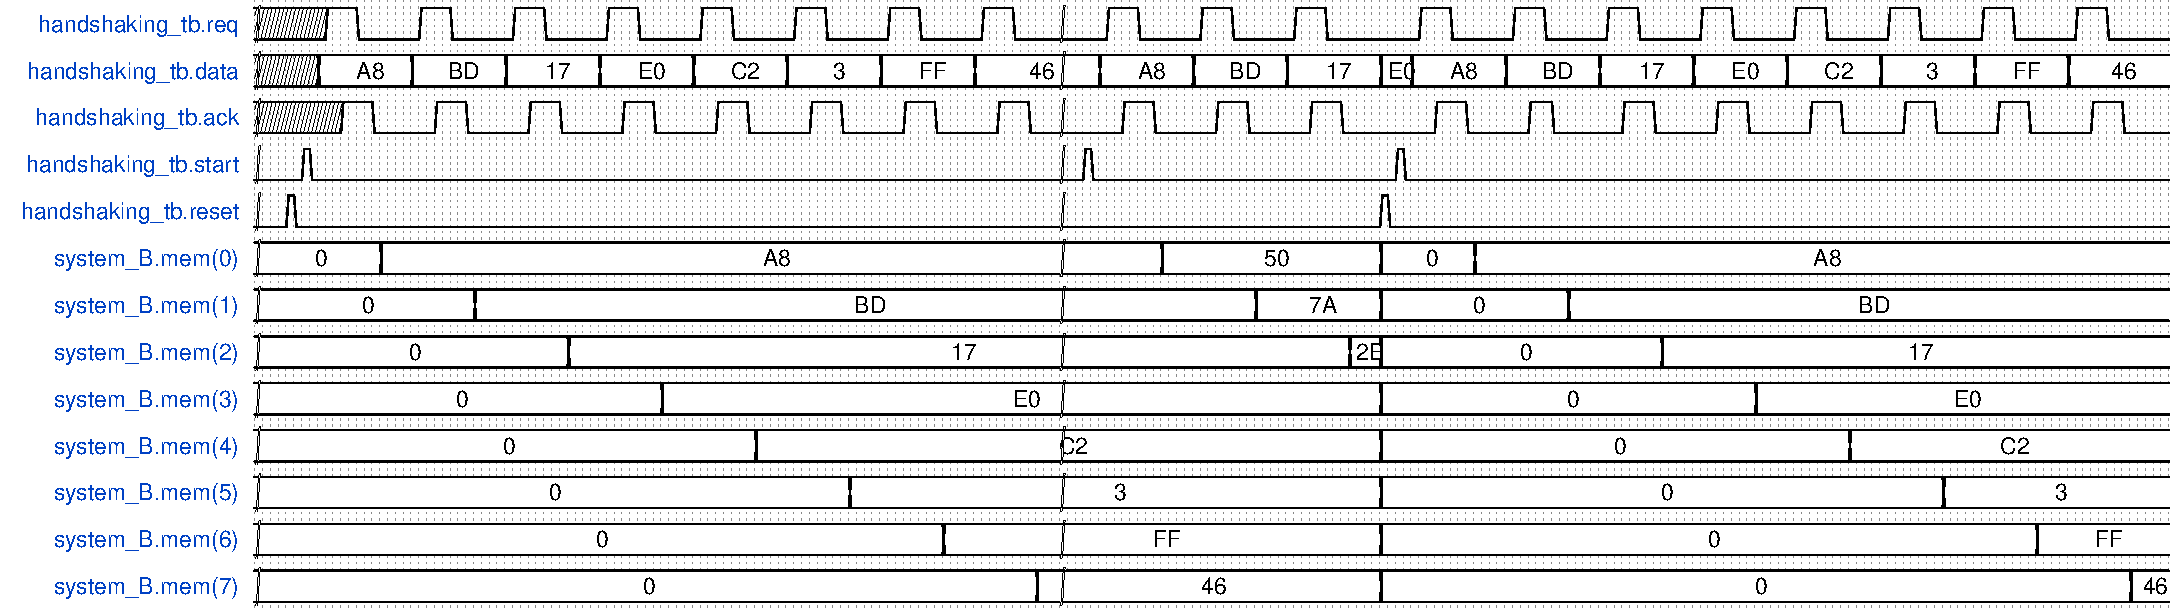
\includegraphics[width=\textwidth]{img/handshaking_tb.pdf}
    \caption{Simulazione del sistema di comunicazione con handshaking}
    \label{fig:handshaking_tb}
\end{figure}